\subsection{Langkah Praktikum: KMP dan Boyer-Moore}
Praktikum 10 mencari pola \texttt{acabaca} pada teks \texttt{abacaabacabacababa}. Algoritma yang digunakan adalah KMP dan Boyer-Moore.

\begin{figure}[H]
    \centering
    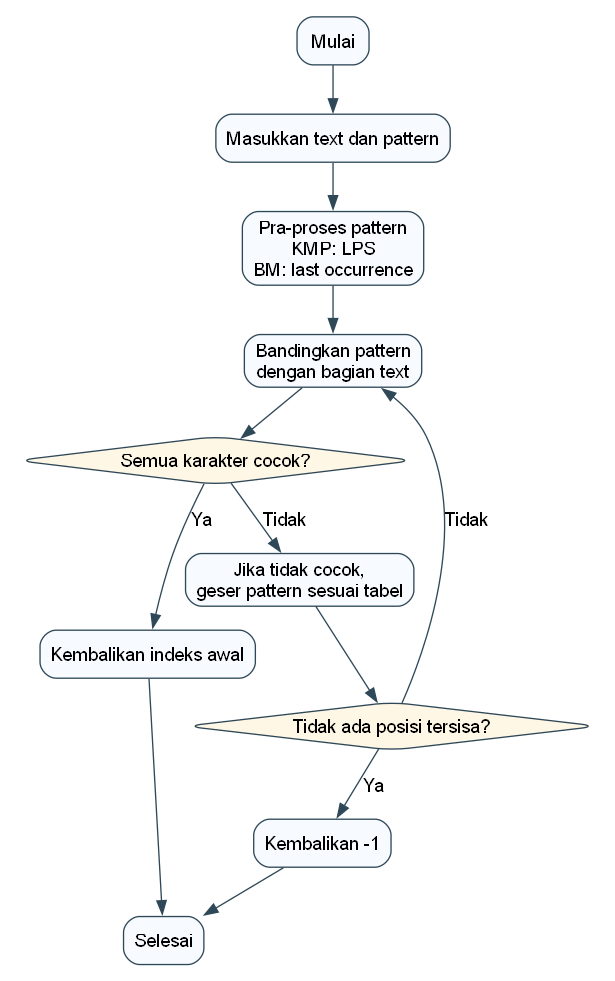
\includegraphics[width=0.62\textwidth]{figures/praktikum10/flowchart_string_matching.png}
    \caption{Flowchart Umum Algoritma String Matching}
    \label{fig:praktikum10-flowchart-string-matching}
\end{figure}

\subsubsection*{Source Code Python}
Source code lengkap terdapat pada folder \texttt{src/praktikum10}. Bagian berikut hanya menampilkan inti program.

\textbf{1. Fungsi LPS dan KMP}
\begin{lstlisting}[basicstyle=\ttfamily\scriptsize, frame=single, backgroundcolor=\color{white}, numbers=none, keywordstyle=\color{black}, commentstyle=\color{black}, stringstyle=\color{black}, breaklines=true]
def compute_lps(pattern):
    lps = [0] * len(pattern)
    prefix_len = 0
    index = 1

    while index < len(pattern):
        if pattern[index] == pattern[prefix_len]:
            prefix_len += 1
            lps[index] = prefix_len
            index += 1
        elif prefix_len != 0:
            prefix_len = lps[prefix_len - 1]
        else:
            lps[index] = 0
            index += 1

    return lps

def kmp_match(text, pattern):
    lps = compute_lps(pattern)
    text_index = 0
    pattern_index = 0

    while text_index < len(text):
        if text[text_index] == pattern[pattern_index]:
            text_index += 1
            pattern_index += 1
            if pattern_index == len(pattern):
                return text_index - pattern_index
        elif pattern_index != 0:
            pattern_index = lps[pattern_index - 1]
        else:
            text_index += 1

    return -1
\end{lstlisting}

\textbf{2. Fungsi Boyer-Moore}
\begin{lstlisting}[basicstyle=\ttfamily\scriptsize, frame=single, backgroundcolor=\color{white}, numbers=none, keywordstyle=\color{black}, commentstyle=\color{black}, stringstyle=\color{black}, breaklines=true]
def build_last_occurrence(pattern):
    last = {}
    for index, char in enumerate(pattern):
        last[char] = index
    return last

def boyer_moore_match(text, pattern):
    last = build_last_occurrence(pattern)
    start = 0

    while start <= len(text) - len(pattern):
        pattern_index = len(pattern) - 1

        while pattern_index >= 0 and pattern[pattern_index] == text[start + pattern_index]:
            pattern_index -= 1

        if pattern_index < 0:
            return start

        mismatch_char = text[start + pattern_index]
        last_index = last.get(mismatch_char, -1)
        start += max(1, pattern_index - last_index)

    return -1
\end{lstlisting}

\textbf{3. Kode tester}
\begin{lstlisting}[basicstyle=\ttfamily\scriptsize, frame=single, backgroundcolor=\color{white}, numbers=none, keywordstyle=\color{black}, commentstyle=\color{black}, stringstyle=\color{black}, breaklines=true]
if __name__ == "__main__":
    ptext = "abacaabacabacababa"
    pattern = "acabaca"

    print(kmp_match(ptext, pattern))
    print(boyer_moore_match(ptext, pattern))
\end{lstlisting}

\subsubsection*{Analisis}
\textbf{Hasil program:}
\begin{table}[H]
    \centering
    \caption{Hasil Pencocokan String Praktikum 10}
    \label{tab:praktikum10-hasil}
    \begin{tabular}{lll}
    \toprule
    \textbf{Algoritma} & \textbf{Indeks Ditemukan} & \textbf{Keterangan} \\ \midrule
    KMP & 7 & Pola ditemukan. \\
    Boyer-Moore & 7 & Pola ditemukan. \\ \bottomrule
    \end{tabular}
\end{table}

\textbf{Tabel LPS KMP:}
\begin{table}[H]
    \centering
    \caption{Tabel LPS untuk Pola \texttt{acabaca}}
    \label{tab:praktikum10-lps}
    \begin{tabular}{cccccccc}
    \toprule
    \textbf{Indeks} & 0 & 1 & 2 & 3 & 4 & 5 & 6 \\ \midrule
    \textbf{Karakter} & a & c & a & b & a & c & a \\
    \textbf{LPS} & 0 & 0 & 1 & 0 & 1 & 2 & 3 \\ \bottomrule
    \end{tabular}
\end{table}

\begin{figure}[H]
    \centering
    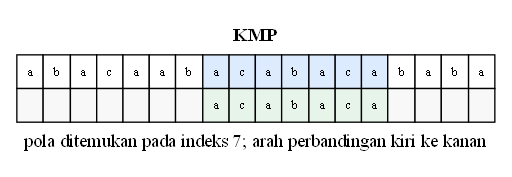
\includegraphics[width=0.86\textwidth]{figures/praktikum10/kmp_match.png}
    \caption{Hasil Pencocokan Pola Menggunakan KMP}
    \label{fig:praktikum10-kmp-match}
\end{figure}

\begin{figure}[H]
    \centering
    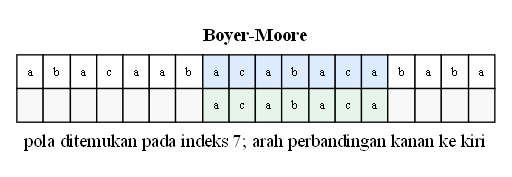
\includegraphics[width=0.86\textwidth]{figures/praktikum10/boyer_moore_match.png}
    \caption{Hasil Pencocokan Pola Menggunakan Boyer-Moore}
    \label{fig:praktikum10-boyer-moore-match}
\end{figure}

\textbf{Post Test: Implementasi Boyer-Moore}
\begin{table}[H]
    \centering
    \caption{Validasi KMP dan Boyer-Moore pada Kasus yang Sama}
    \label{tab:praktikum10-validasi-posttest}
    \begin{tabular}{llll}
    \toprule
    \textbf{Text} & \textbf{Pattern} & \textbf{KMP} & \textbf{Boyer-Moore} \\ \midrule
    \texttt{abacaabacabacababa} & \texttt{acabaca} & 7 & 7 \\ \bottomrule
    \end{tabular}
\end{table}

\textbf{Kesimpulan:} KMP dan Boyer-Moore sama-sama menemukan pola pada indeks 7. Hasil post test sesuai karena Boyer-Moore memberikan posisi yang sama dengan KMP.
